%!TEX root = ../../../adrien_gomar_phd.tex

\subsection{Similarity coefficients}
\label{sub:dream_ls_hb_sim_coeff}

Figure~\ref{fig:dream_ls_hb_unst_coeff} depicts the
unsteady variation of the thrust coefficient $C_T$ on 
both the front and the rear rotor.
The time is 
normalized by the reference period of the current rotor 
(the rotation frequency~$n$) and the thrust coefficient is normalized
by its temporal mean value. This allow to assess the unsteady variations
over one reference period. 


The level of unsteadiness is rather
the same on both rotors as it represents an envelope of almost
1\% of the temporal mean value. This level is not negligible and
justifies the use of unsteady methods on CROR configurations. 
Moreover, even though wakes are shed behind the front rotor
that impinge the rear rotor blades, the level of unsteadiness
perceived by the rear rotor is close to the front rotor ones.
\begin{figure}[htp]
  \centering
  \subfigure[front rotor]{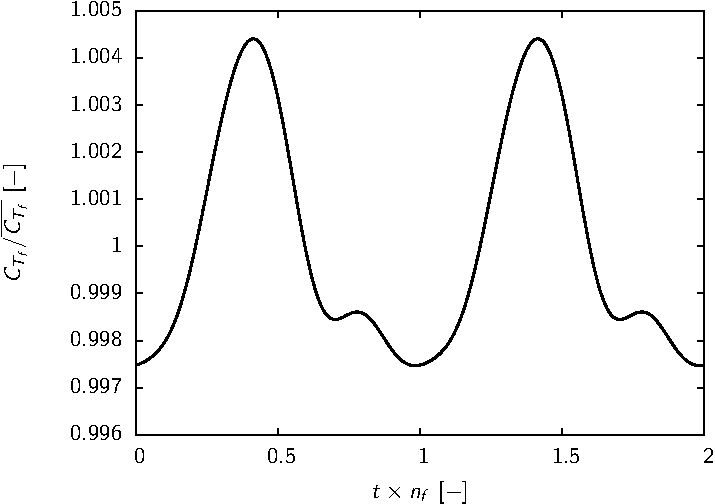
\includegraphics[width=.35\textwidth]{DREAM_LS_TSM_FORCES_INST_FRONT_PPT.pdf}}
  \subfigure[rear rotor]{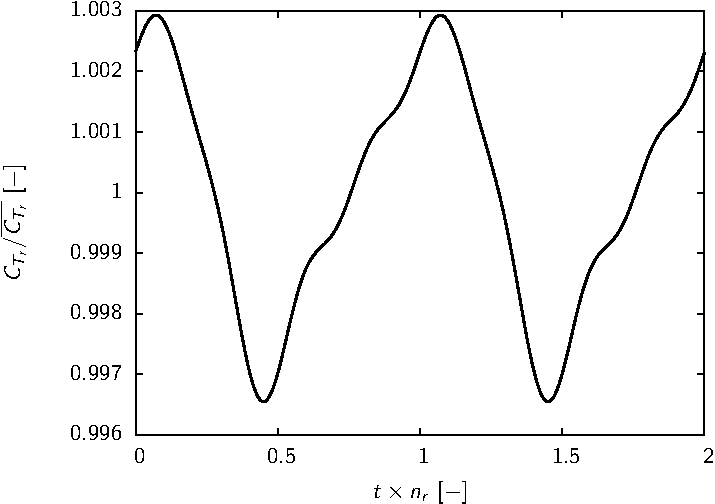
\includegraphics[width=.35\textwidth]{DREAM_LS_TSM_FORCES_INST_REAR_PPT.pdf}}
  \caption{Low-speed isolated configuration: unsteadiness seen by the rotors.}
  \label{fig:dream_ls_hb_unst_coeff}
\end{figure}

To assess in more detail the unsteady flow
field seen by the blade, an harmonic analysis on the
blades is performed in the following section.

\subsection{Two-dimensional results: harmonic blade response}
\label{sub:dream_ls_hb_blade_response}

A discrete Fourier transform is post-processed on the blades
for the unsteady static pressure variable. This gives an
idea of the level of unsteadiness seen locally by the blades.
The amplitude is shown in 
Fig.~\ref{fig:dream_ls_hb_blade_response} for both blades.
The legend is in logarithmic scale and it is different
for the front and rear rotor blades. In fact, even though the
integrated level of unsteadiness is relatively the same, this
fails when looking at local results. Roughly, the harmonic
amplitude of the static pressure on the rear rotor is
ten times larger.
\begin{figure}[htp]
 \ra{1.3} \centering
 \begin{tabular}{cccc}
    \multicolumn{2}{c}{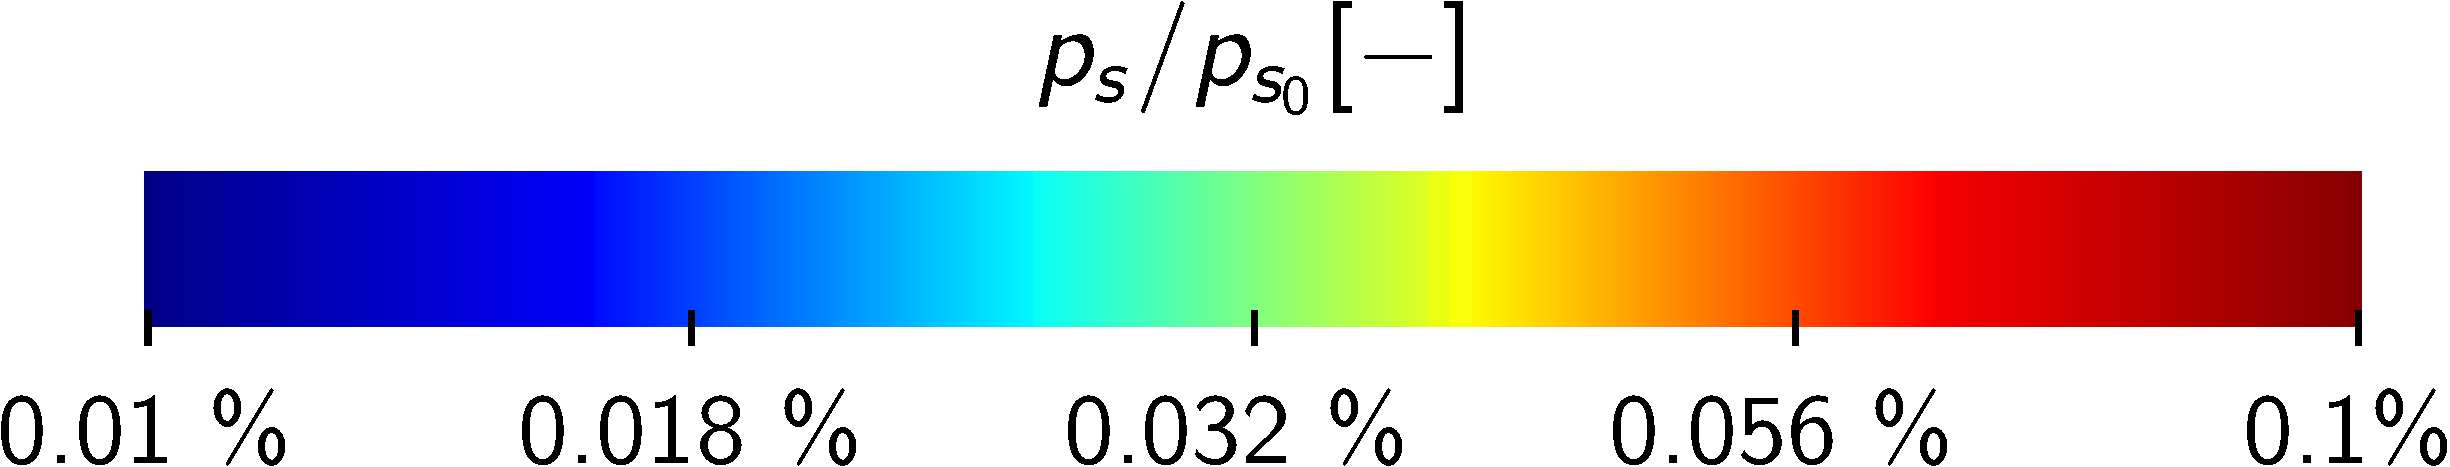
\includegraphics[width=0.3\textwidth]{dream_ls_blade_resp_scale_H01_front.pdf}} &
    \multicolumn{2}{c}{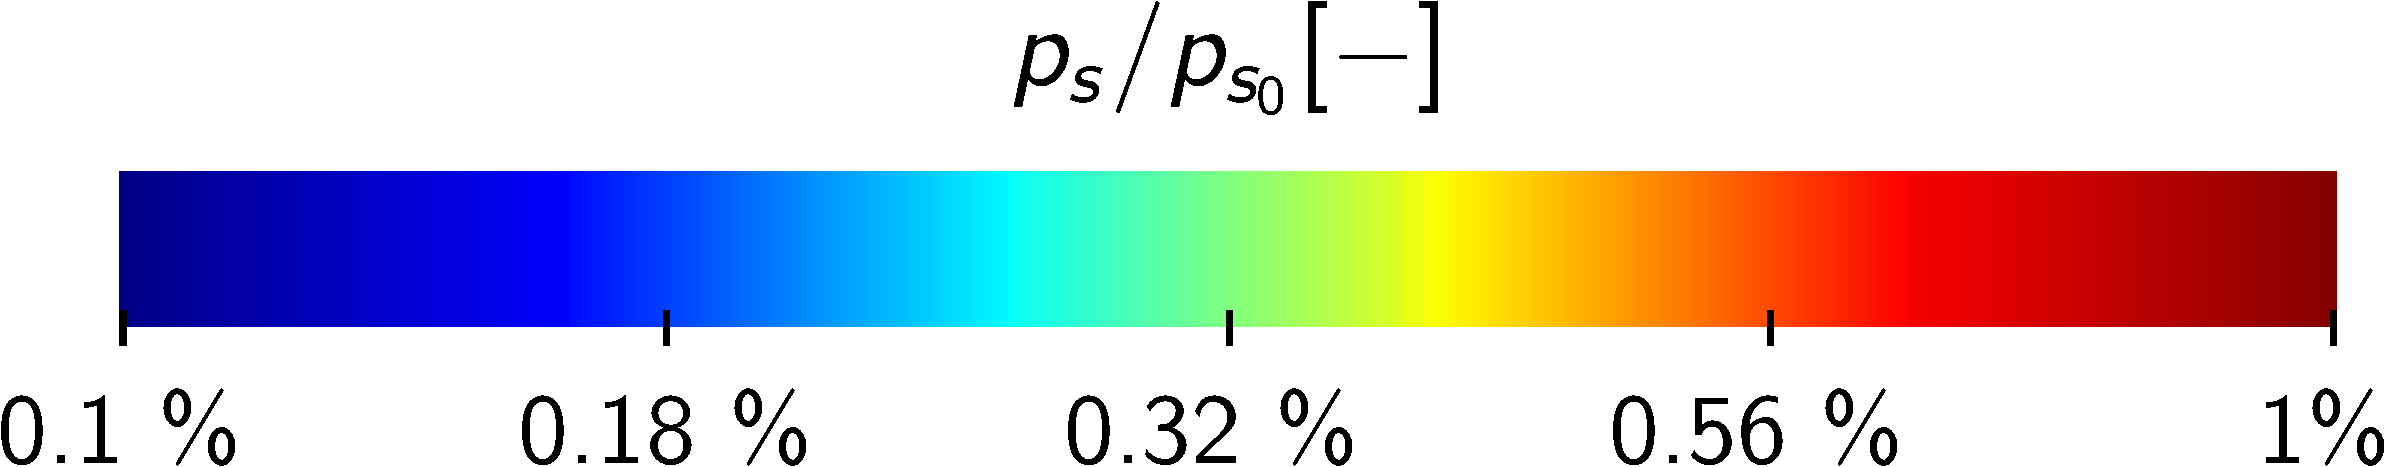
\includegraphics[width=0.3\textwidth]{dream_ls_blade_resp_scale_H01_rear.pdf}} \\
    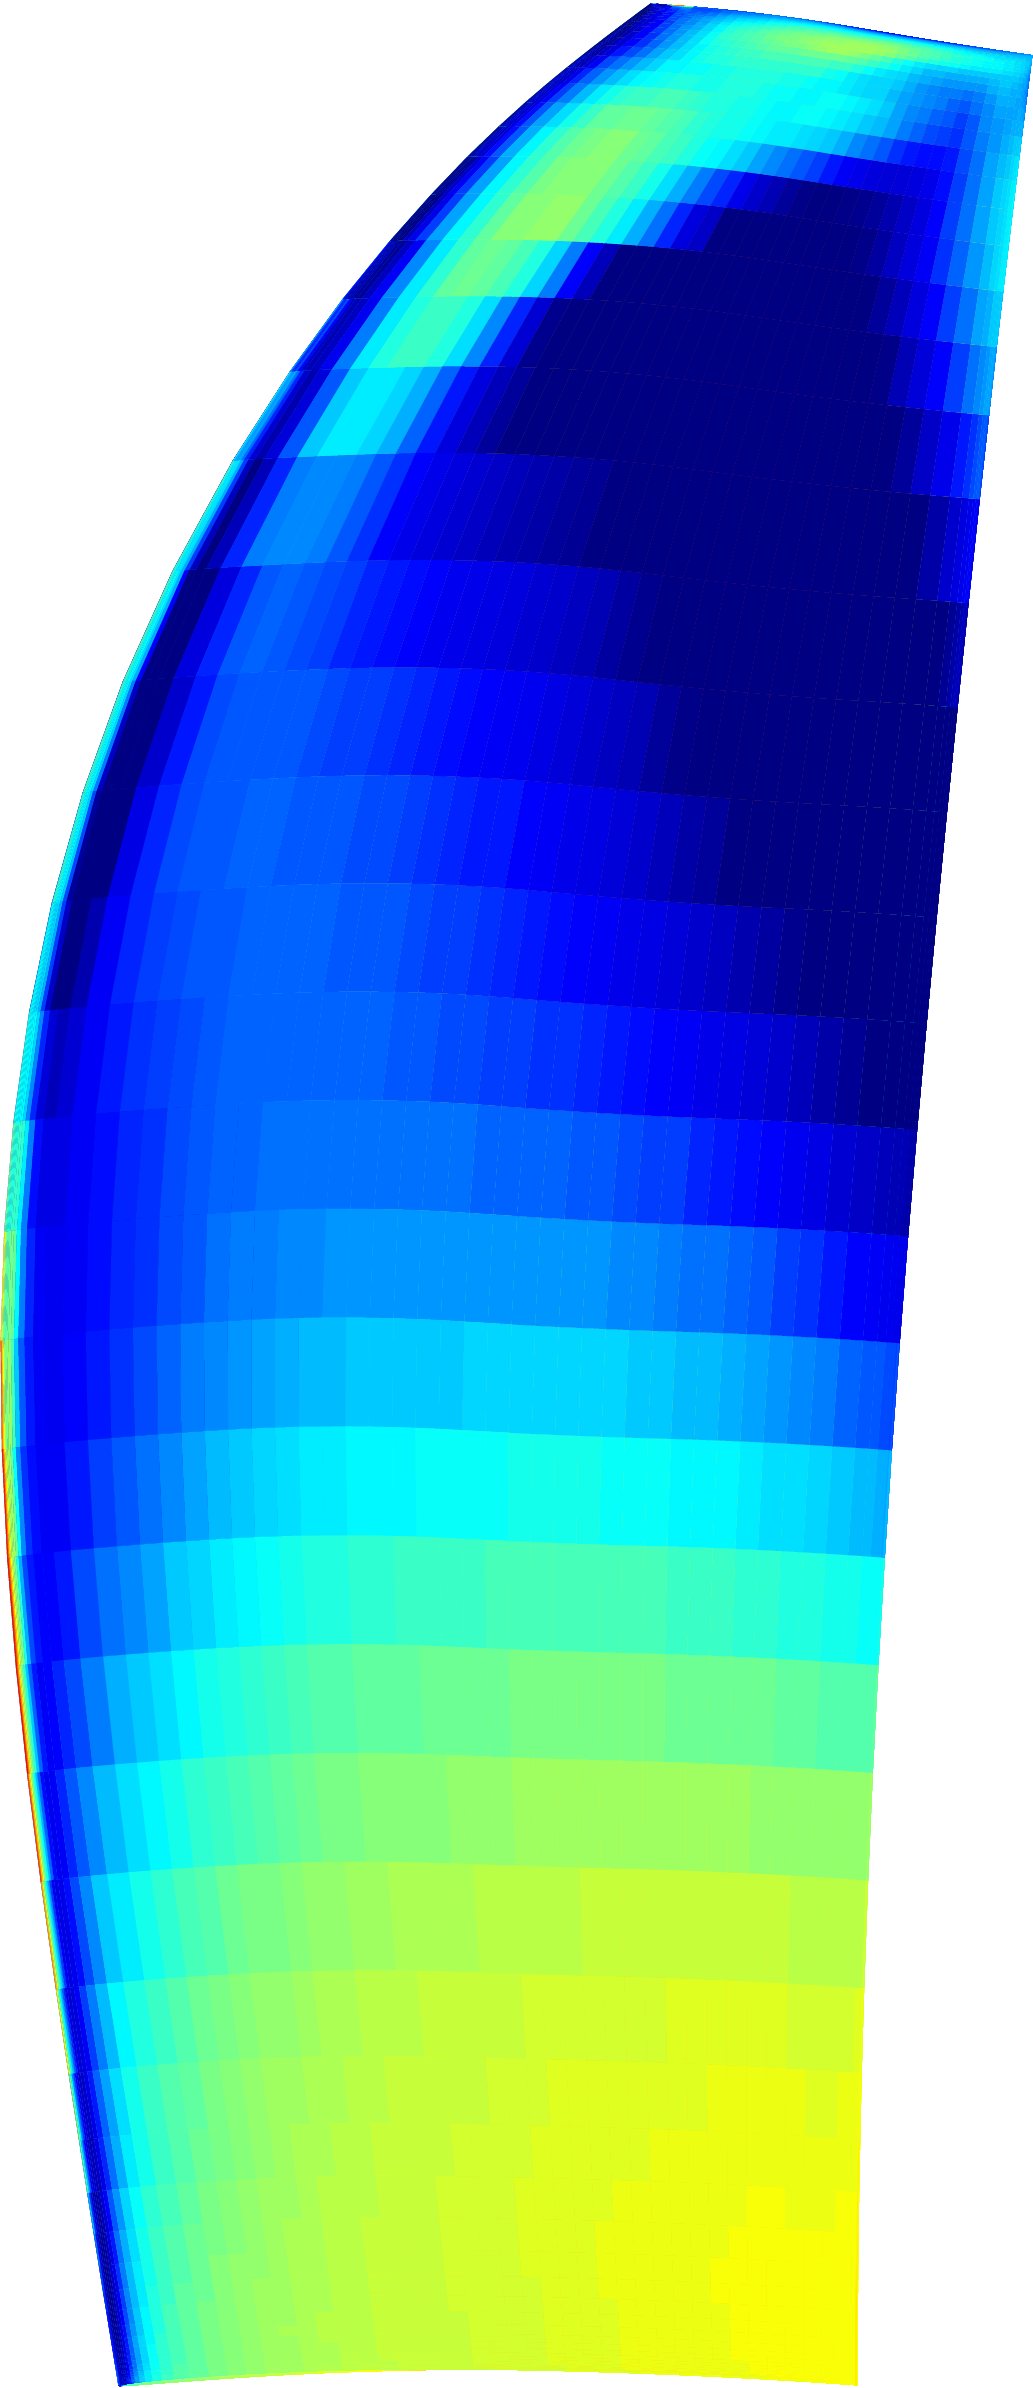
\includegraphics[width=0.15\textwidth]{DREAM_LS_TSM_N4_roe2_sa_blade_response_front_H01_SS.png}
    & 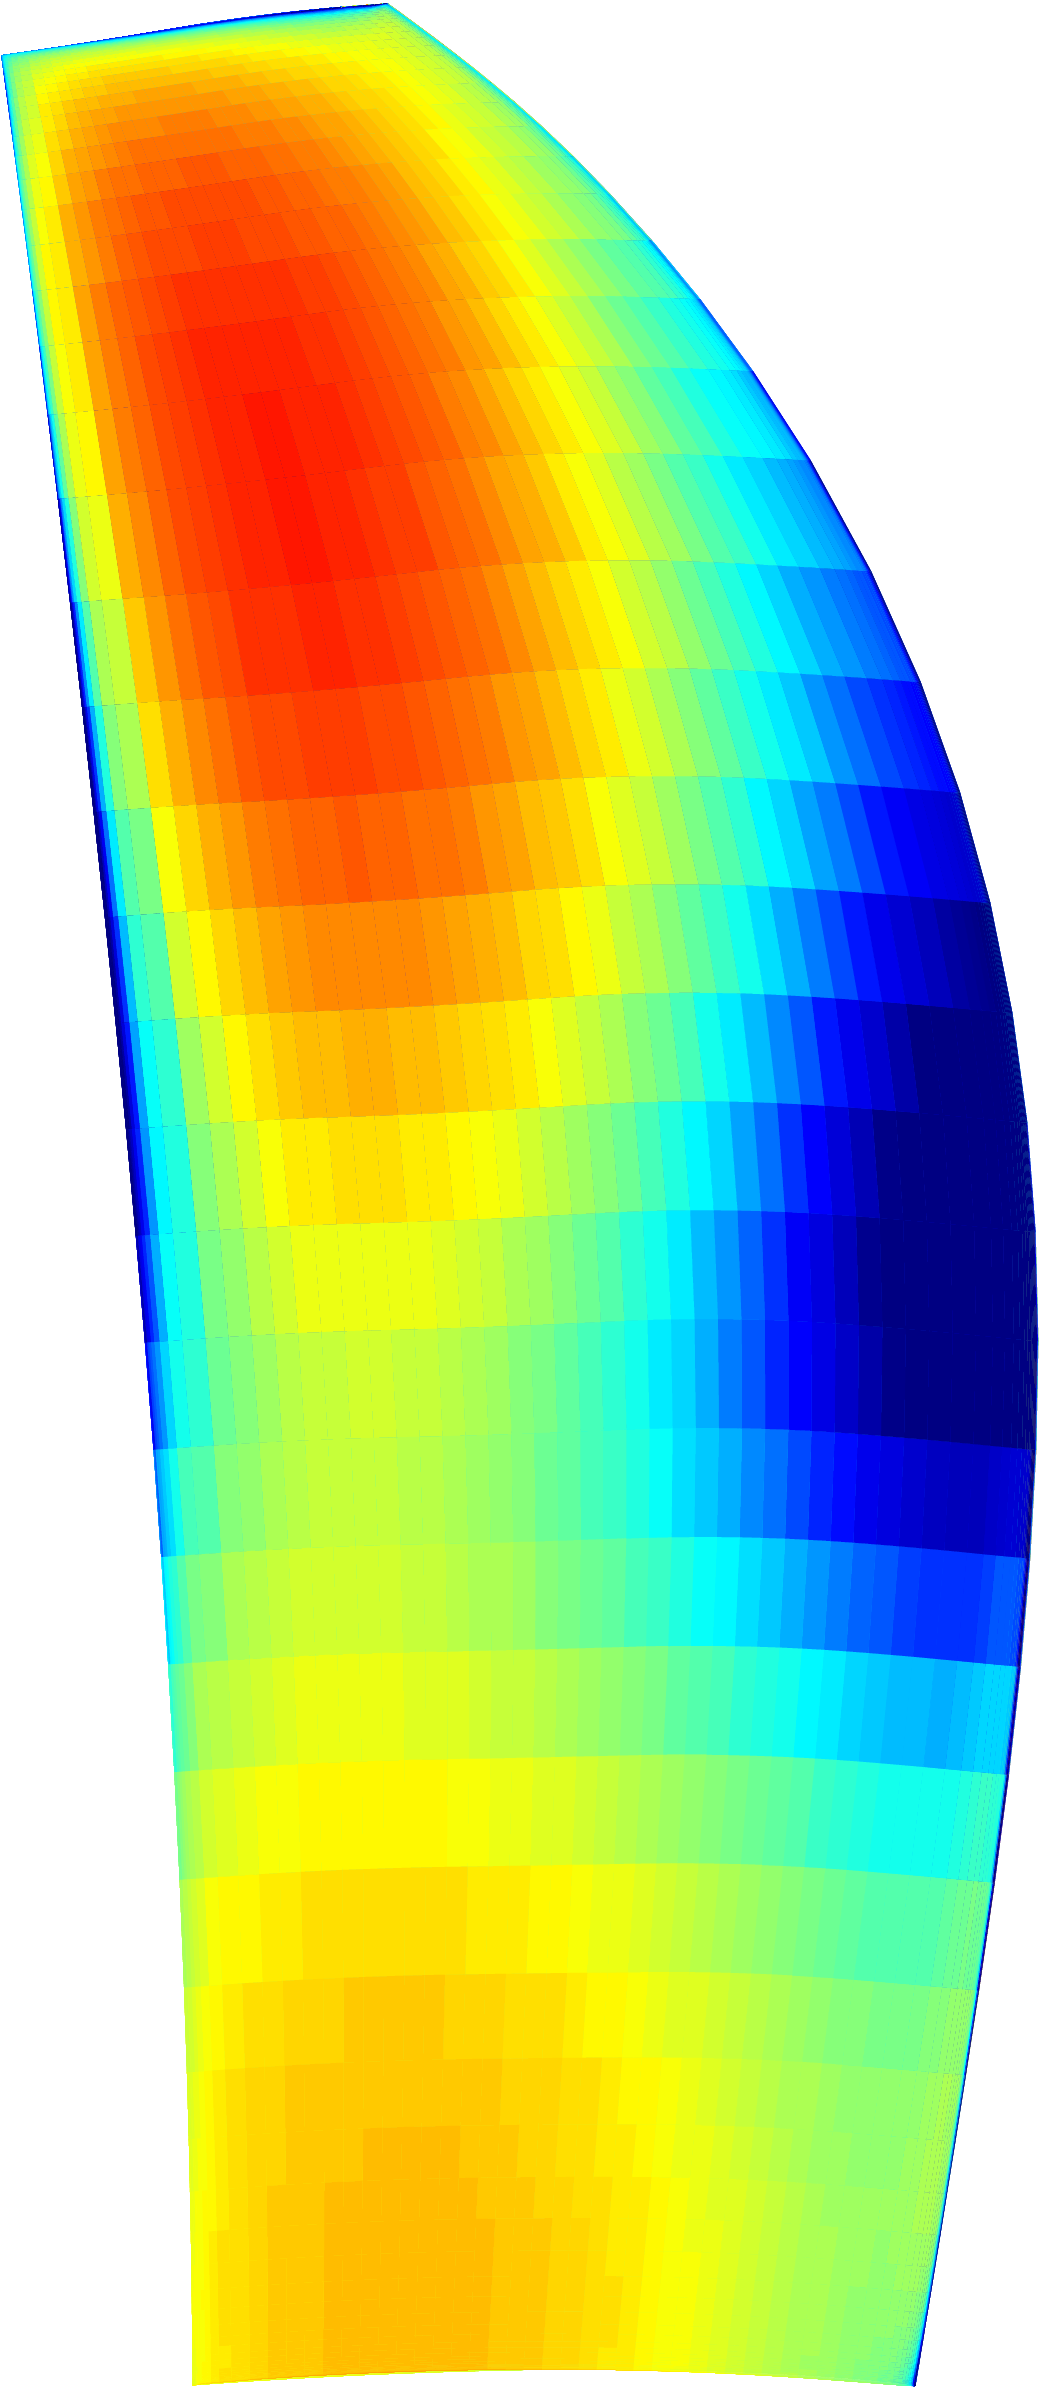
\includegraphics[width=0.15\textwidth]{DREAM_LS_TSM_N4_roe2_sa_blade_response_front_H01_PS.png}
    & 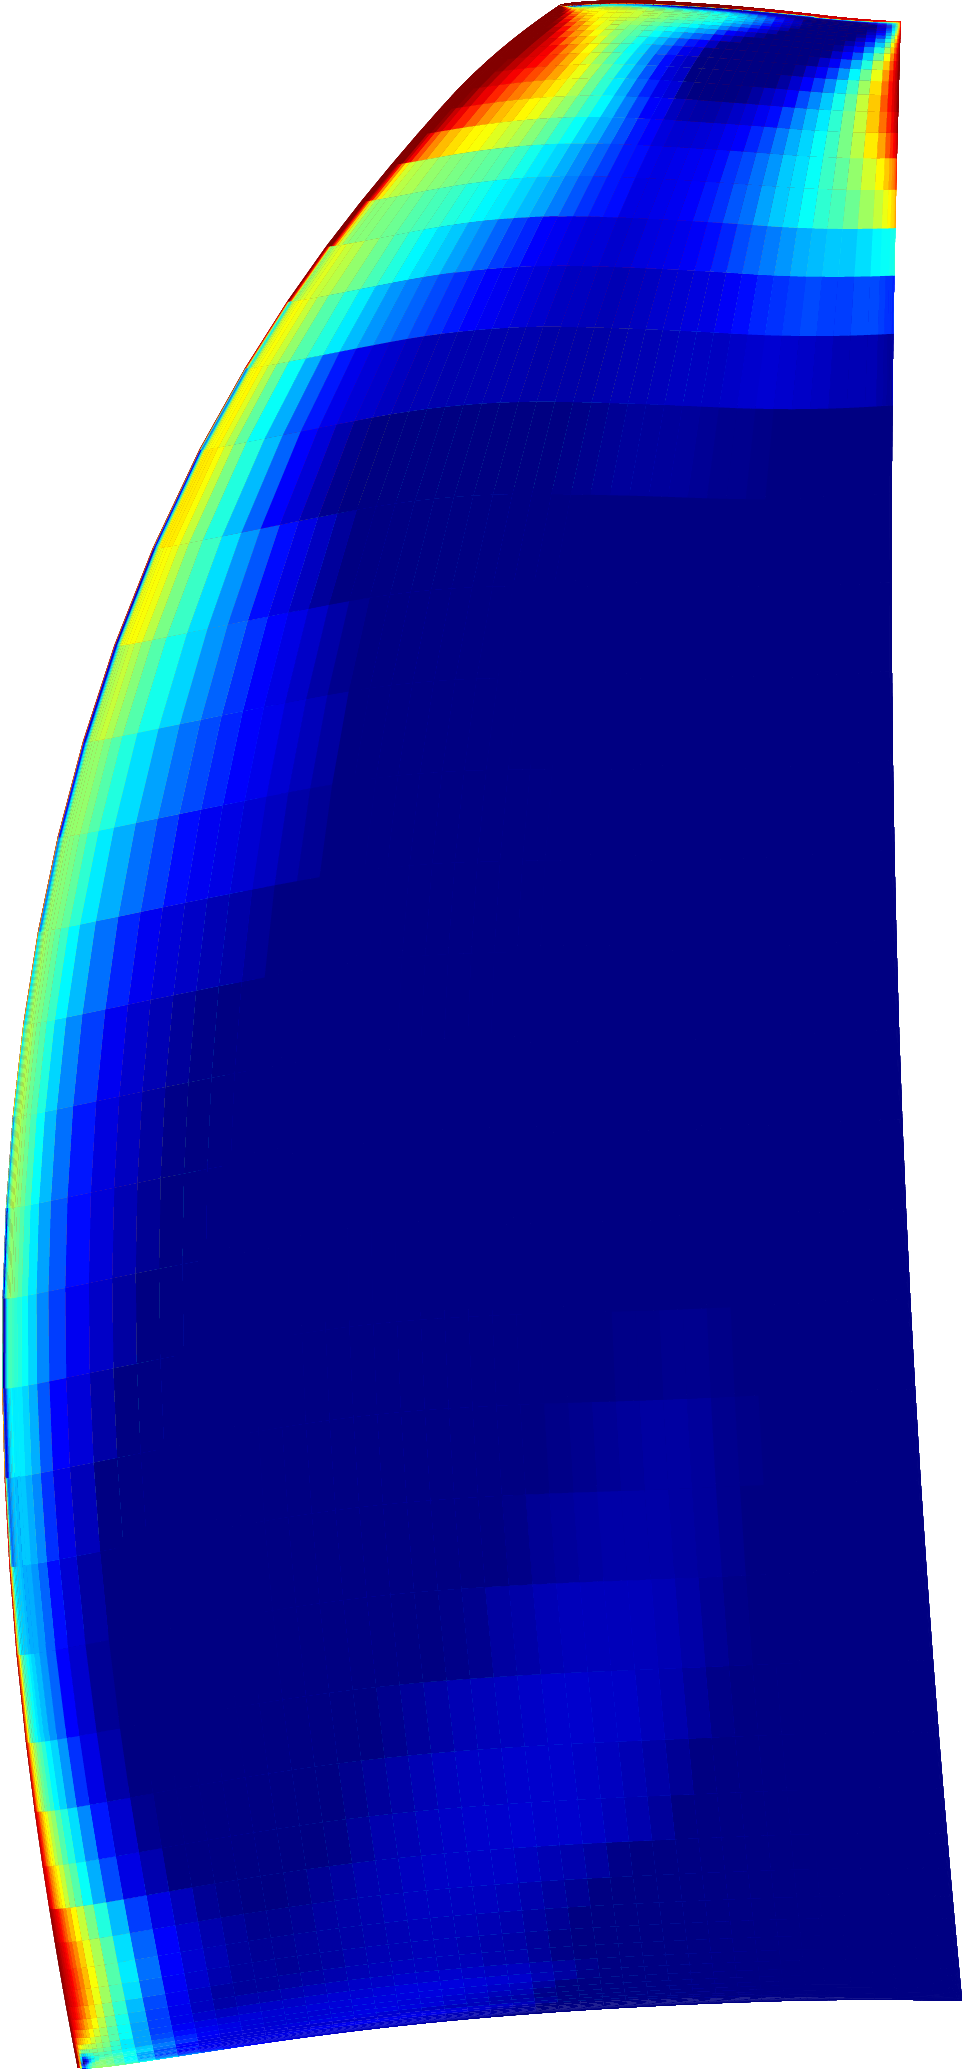
\includegraphics[width=0.15\textwidth]{DREAM_LS_TSM_N4_roe2_sa_blade_response_rear_H01_PS.png}
    & 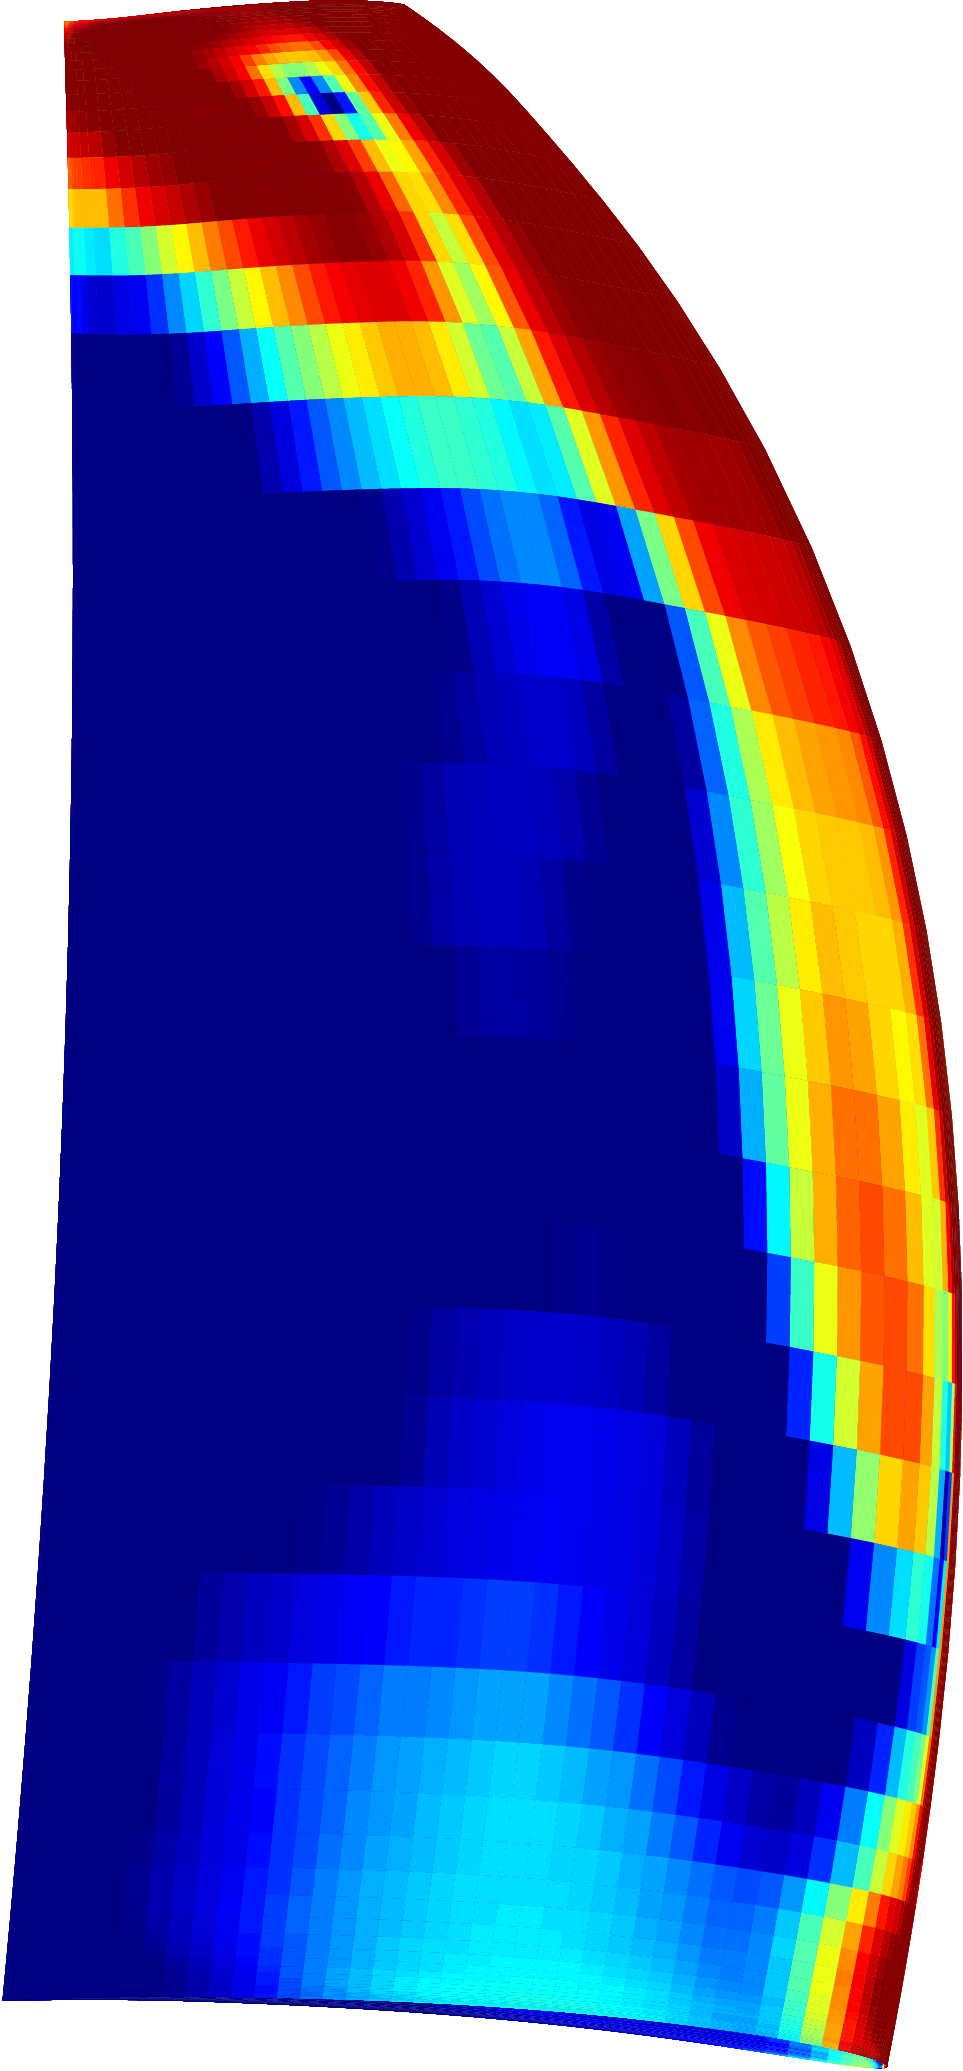
\includegraphics[width=0.15\textwidth]{DREAM_LS_TSM_N4_roe2_sa_blade_response_rear_H01_SS.png} \\
    \multicolumn{2}{c}{\emph{Front rotor blade}}
    & \multicolumn{2}{c}{\emph{Rear rotor blade}} \\
    suction side & pressure side & pressure side & suction side
 \end{tabular}
 \caption{Low-speed isolated configuration: harmonic response of the front
 rotor blades.}
 \label{fig:dream_ls_hb_blade_response}
\end{figure}

On the front rotor blade, the level is large as it is
close to $0.1\%$ of the inflow static pressure.
Moreover, the pressure side
exhibits a larger level of unsteadiness compared to the
suction side. This is due to the relative position of the
blades which makes the pressure side more vulnerable to
potential effects. In fact, as can be seen on radial cuts
(as for instance in Fig.~\ref{fig:dream_ls_hb_slice_r_conv})
the suction is shield from the flow
field coming from downstream. The intensity is not
uniform along span with a relatively higher amplitude of
unsteadiness at the tip of the blade and near the hub
on the pressure side. On the suction side, the largest level
of unsteadiness is observed near the hub.

On the rear rotor blade, the level
of unsteadiness is much larger than the one observed on
the front rotor blade. 
Here, the level of unsteadiness
goes up to 1\% of the inflow static pressure.
This is mostly due to the wake passing
shed by the front rotor blades. In fact, on the leading
edge of the suction side of the rear rotor blade, 
a strong harmonic response is observed, while it is 
much smaller on the pressure side. Baring in mind that 
the suction side sees the wake passing, one can deduce
that this strong harmonic response is attributed to wake passing.
In addition to that, in the tip region of the rear rotor blade, 
a stronger level of unsteadiness is observed. As mentioned
previously, tip vortices are shed by the front rotor blades.
Even though the rear rotor blades are clipped, as 
the stream tube contracts, there is a chance that
the front rotor blades tip vortices interact with the 
rear rotor blades. This is investigated by analyzing
axial cuts of entropy.

\subsection{Two-dimensional results: axial cuts}
\label{sub:dream_ls_hb_axial_cuts}

Axial cuts of entropy at four planes ($P3$, $P4$, $P5$ and $P6$)
are shown in Fig.~\ref{fig:dream_ls_hb_axial_cut_entropy}.
Compared to a steady computation, the harmonic balance
approach allows to capture the
tip vortices on the rear rotor. Between plane $P3$
and $P4$, they have been diffused thanks to the viscosity effects.
The interaction of the front and the rear rotor tip vortices
is highlighted in the $P5$ plane. At the end, in plane $P6$
the vortices have almost merged and a large entropy
trace remains. This confirms the impact
of the front rotor tip vortices on the
rear rotor blade, which explains the large static pressure
fluctuations observed in the tip of the rear 
rotor blades.
\begin{figure}[htp]
  \centering
  \subfigure[$P3$]{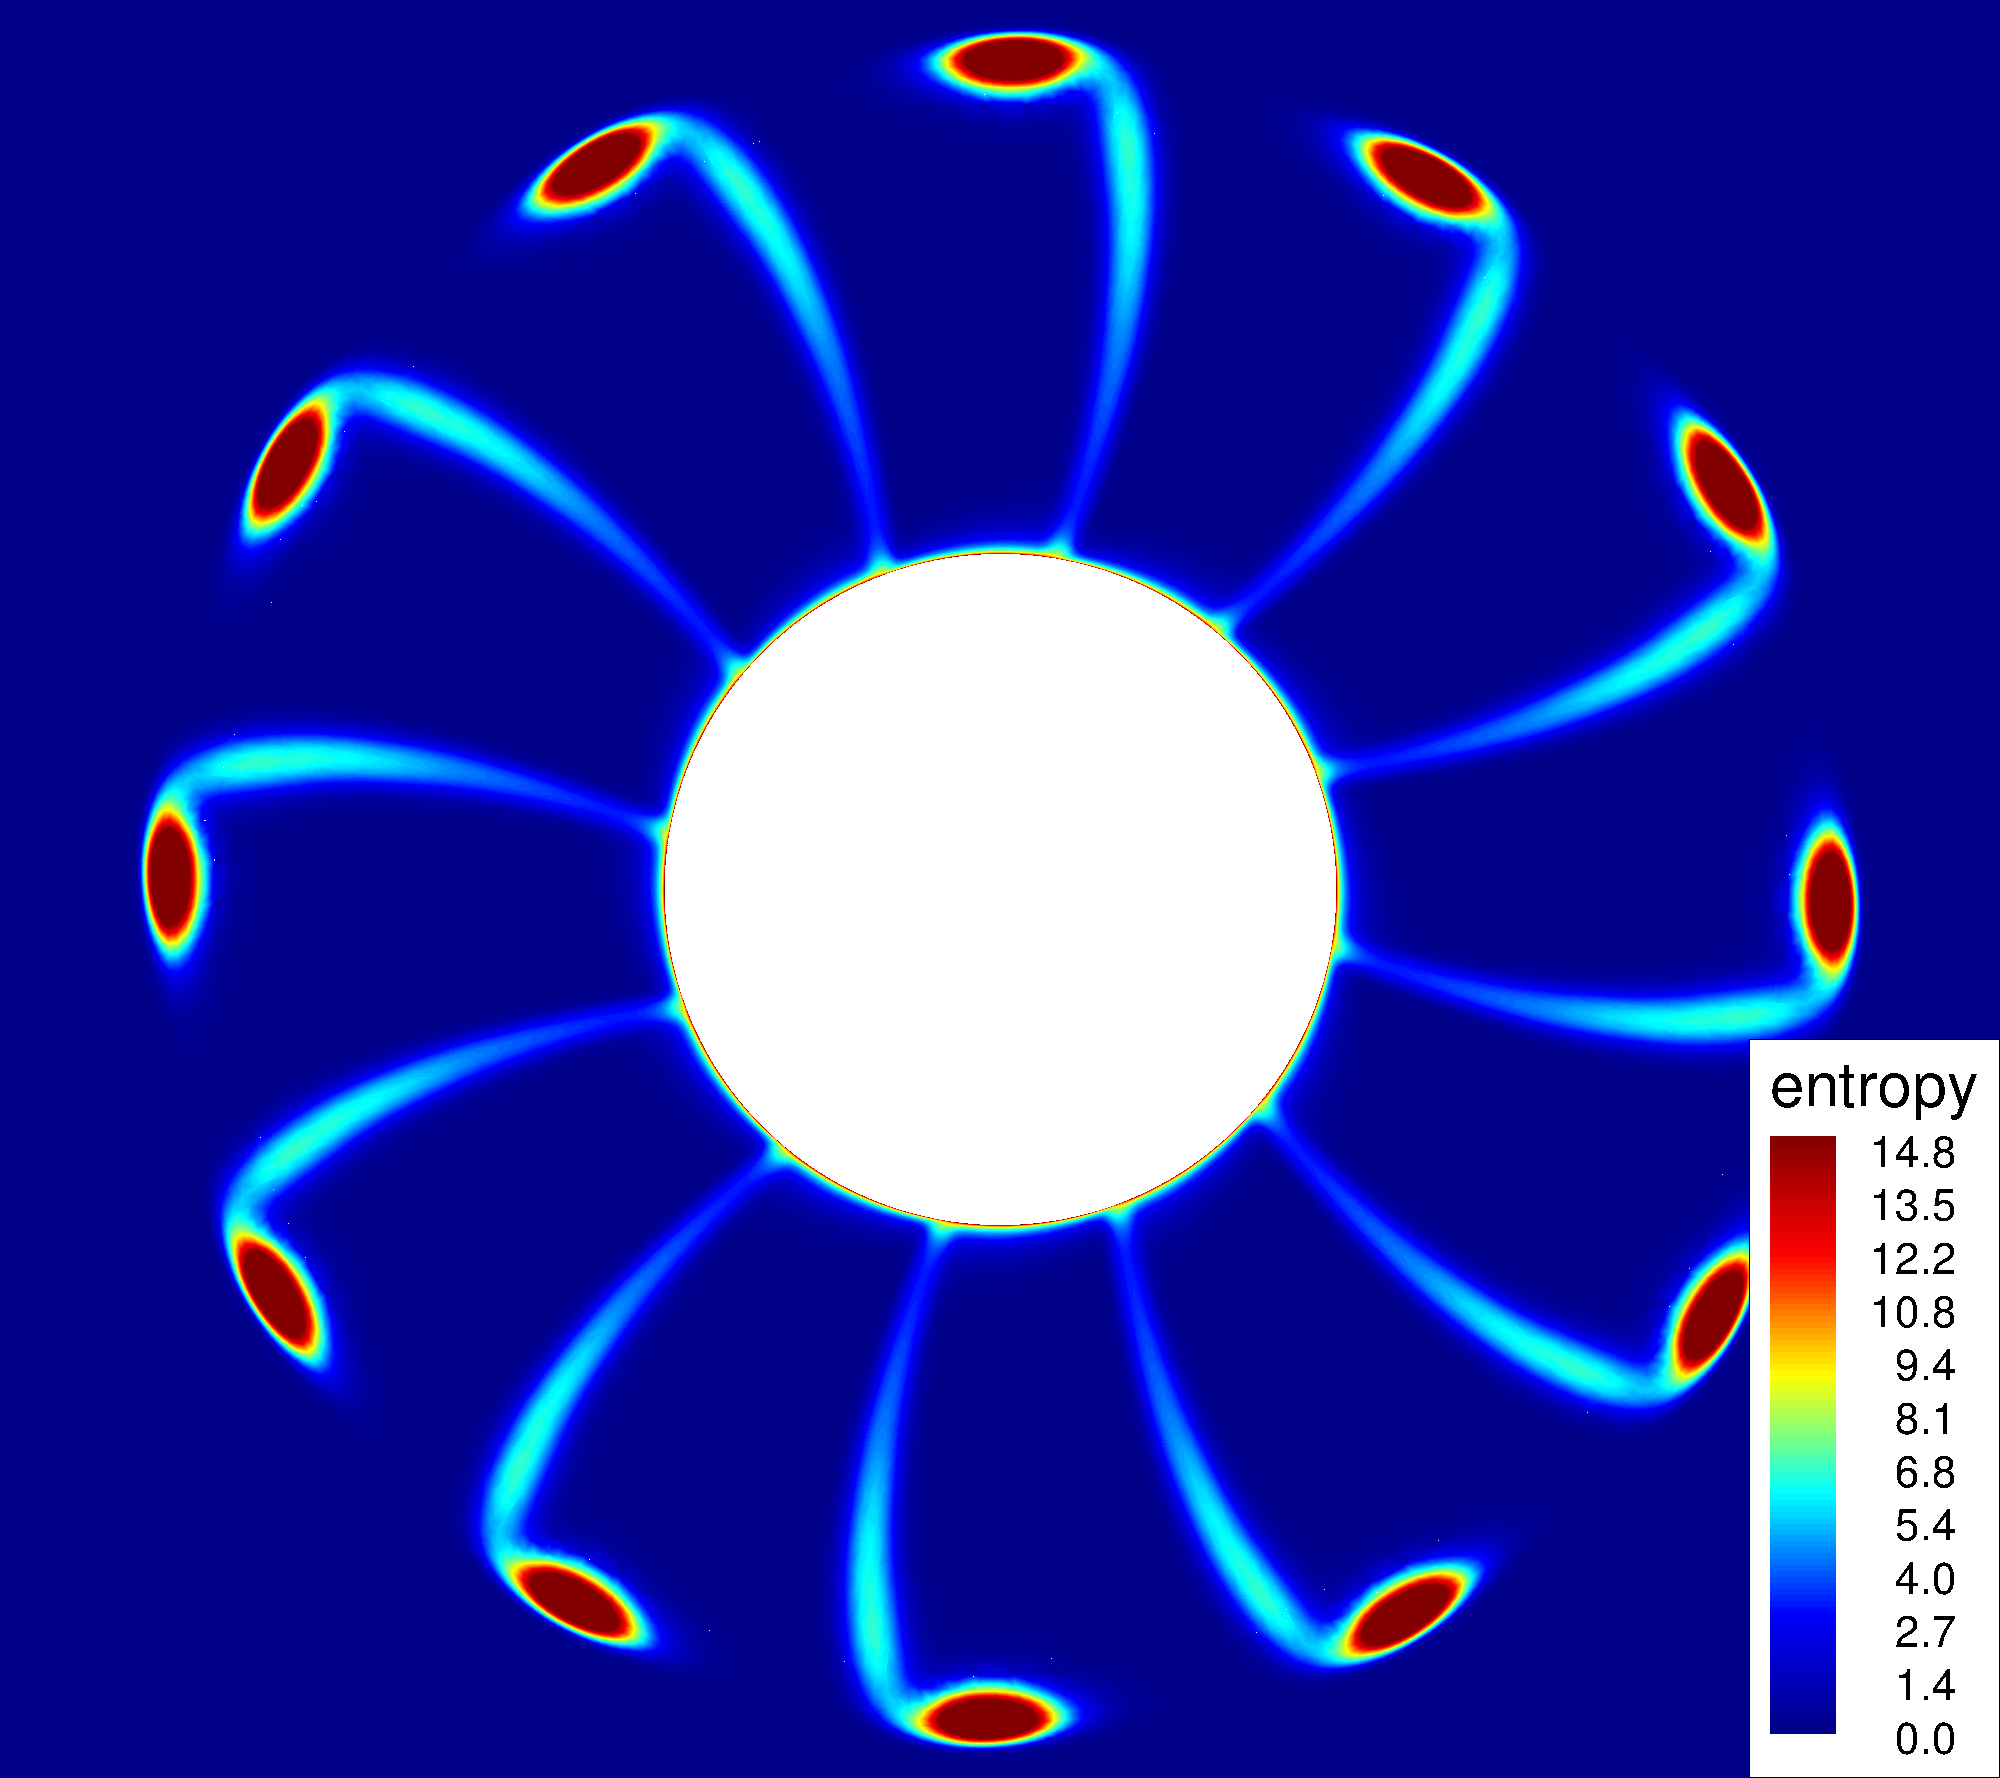
\includegraphics[width=.35\textwidth]{DREAM_LS_TSM_N4_roe2_sa_slice_x_front_1_entropy.png}}
  \subfigure[$P4$]{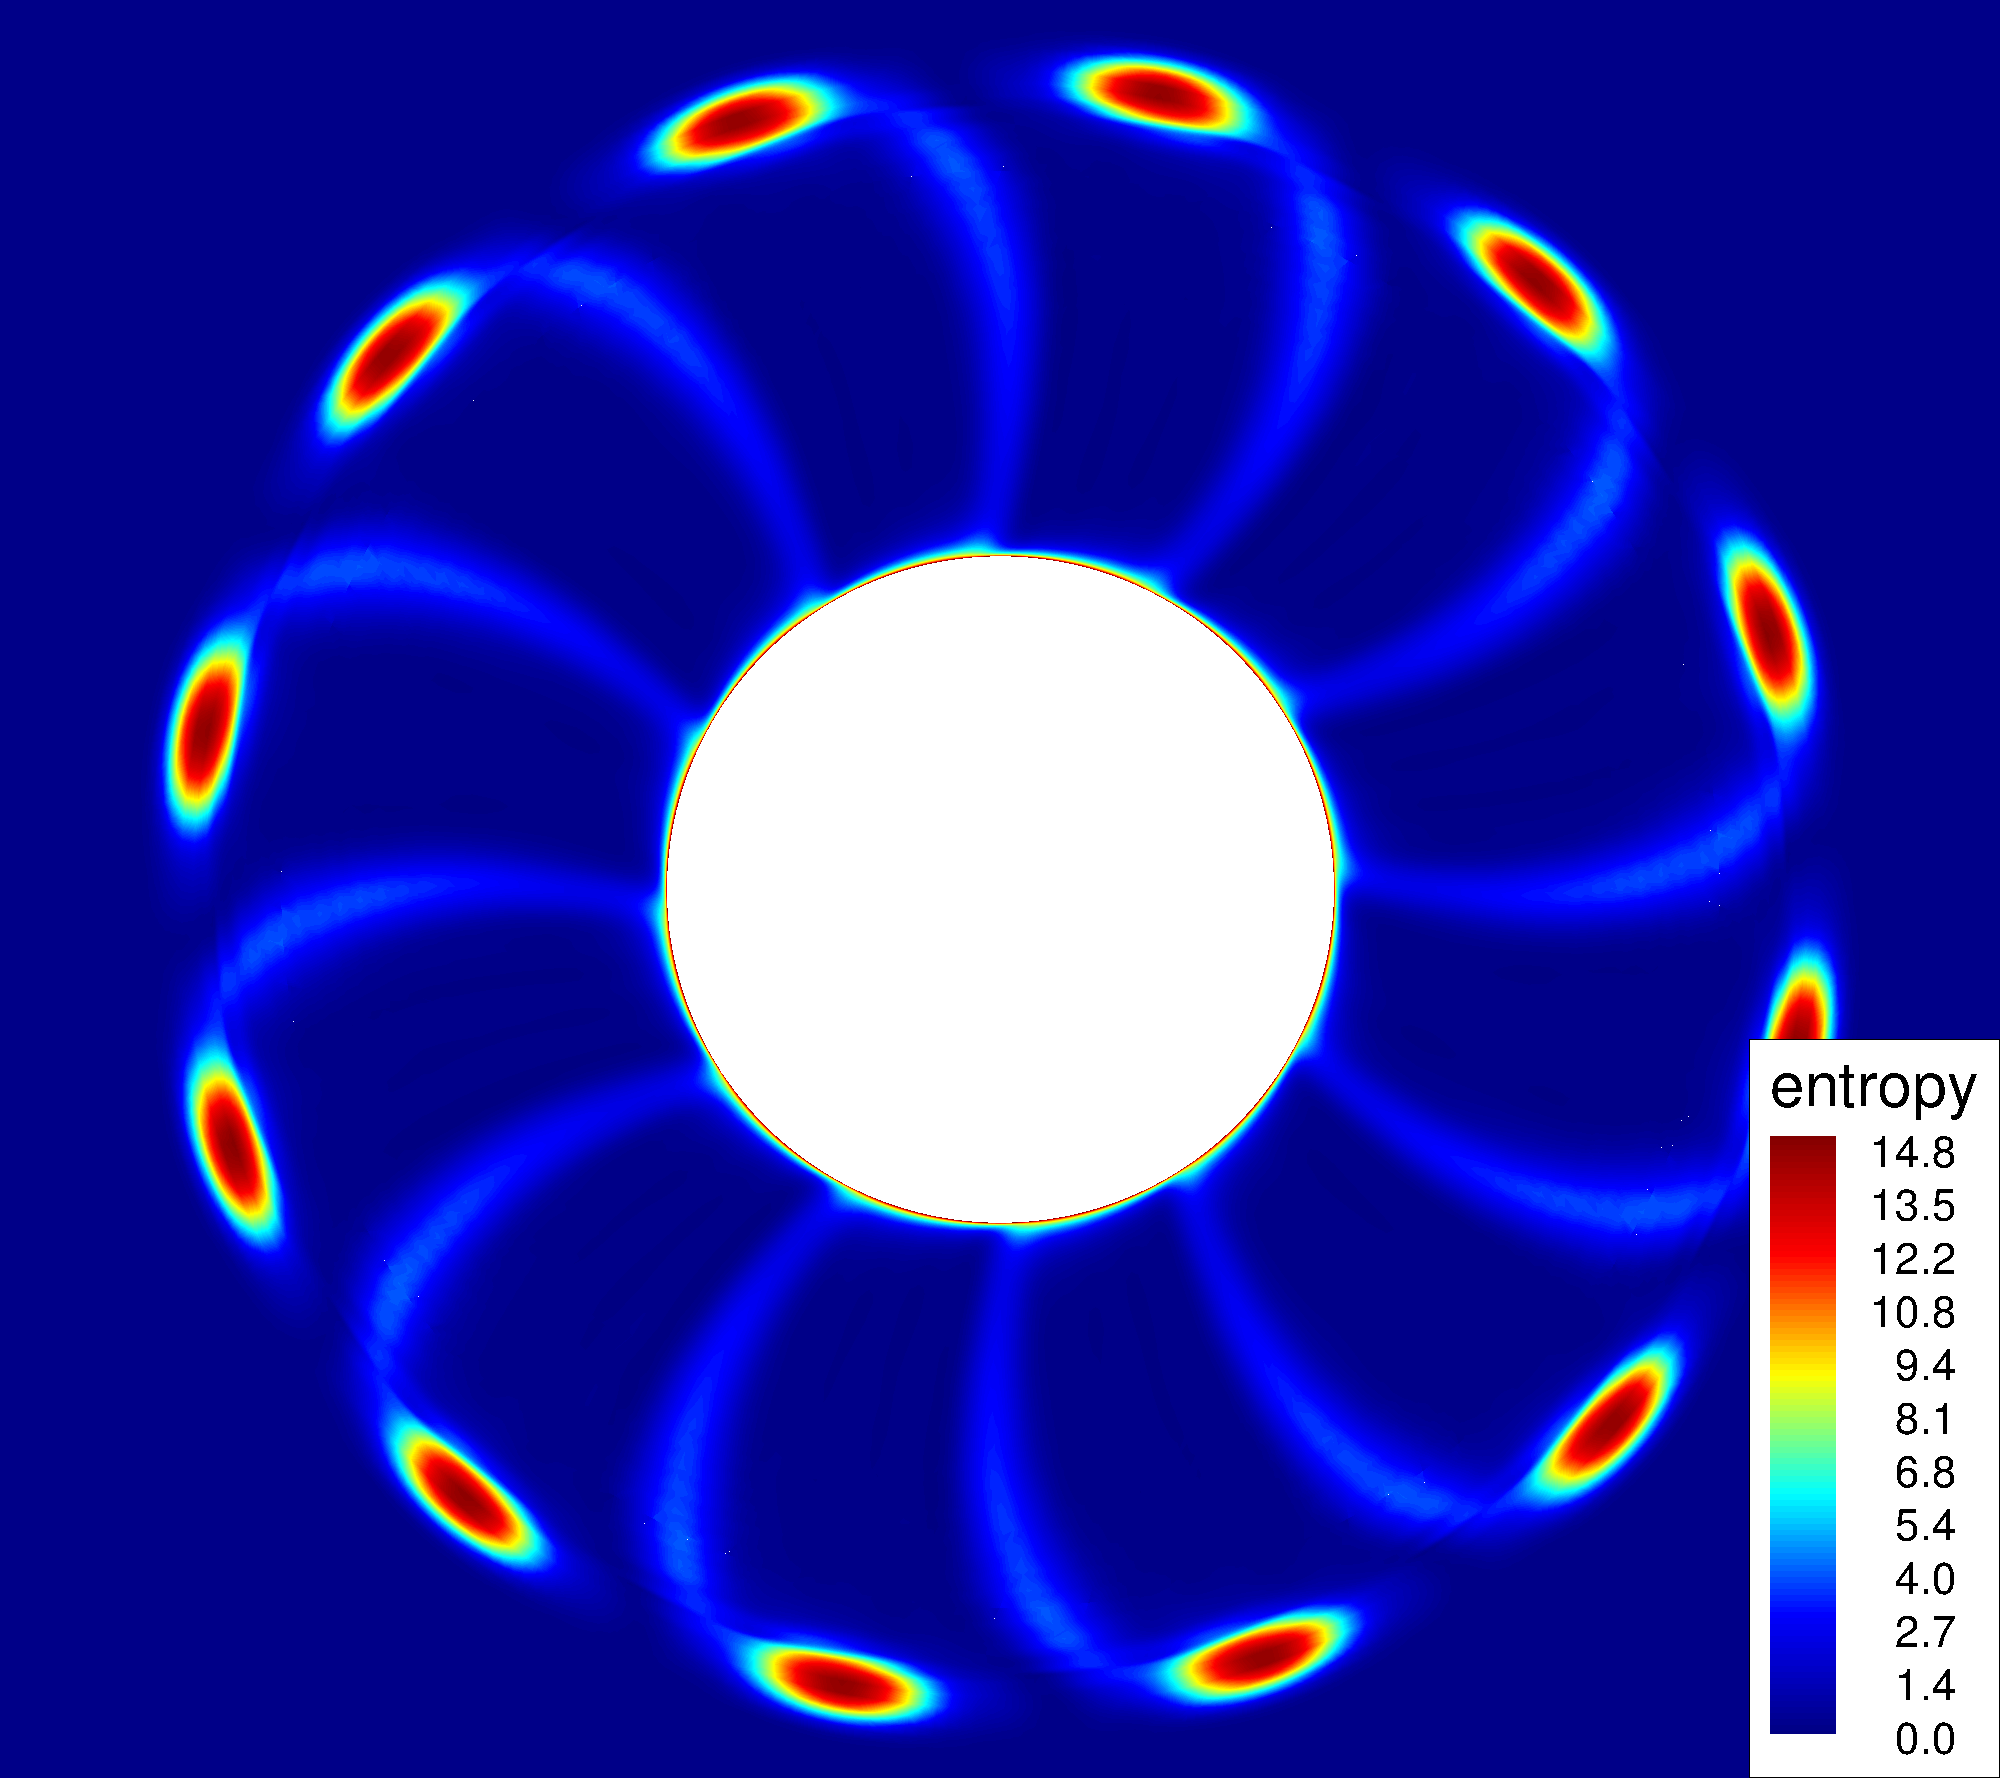
\includegraphics[width=.35\textwidth]{DREAM_LS_TSM_N4_roe2_sa_slice_x_rear_0_entropy.png}}
  \subfigure[$P5$]{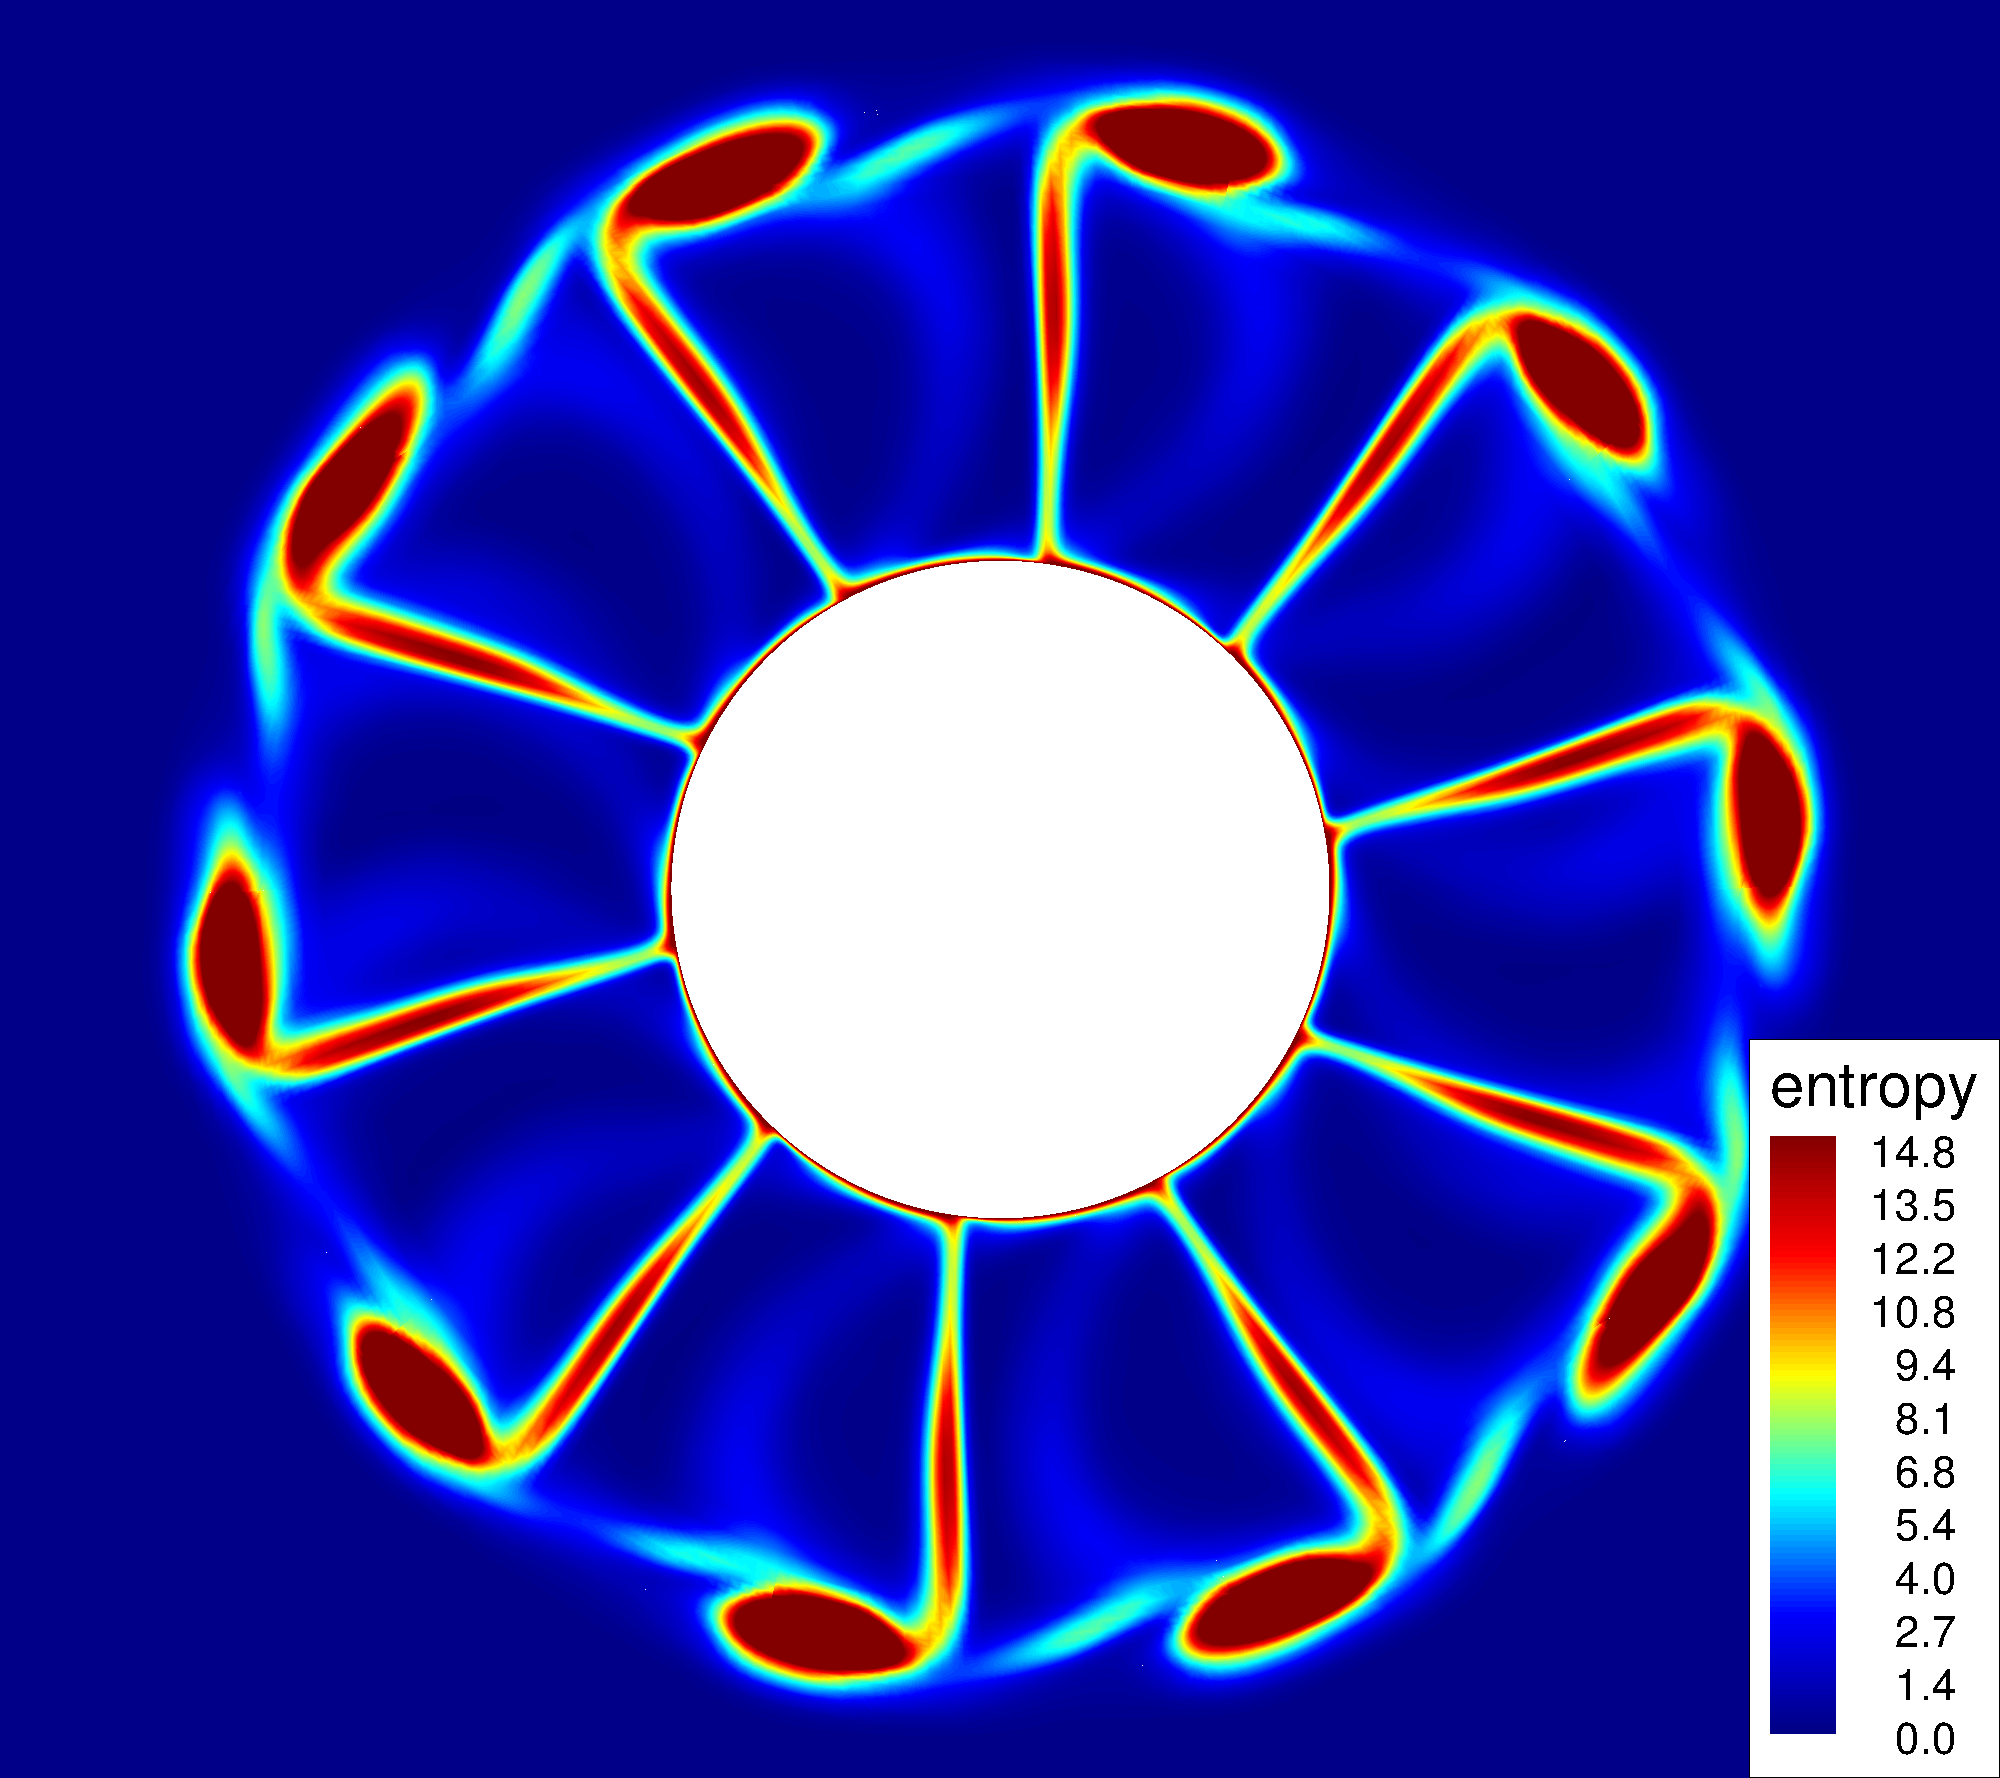
\includegraphics[width=.35\textwidth]{DREAM_LS_TSM_N4_roe2_sa_slice_x_rear_1_entropy.png}}
  \subfigure[$P6$]{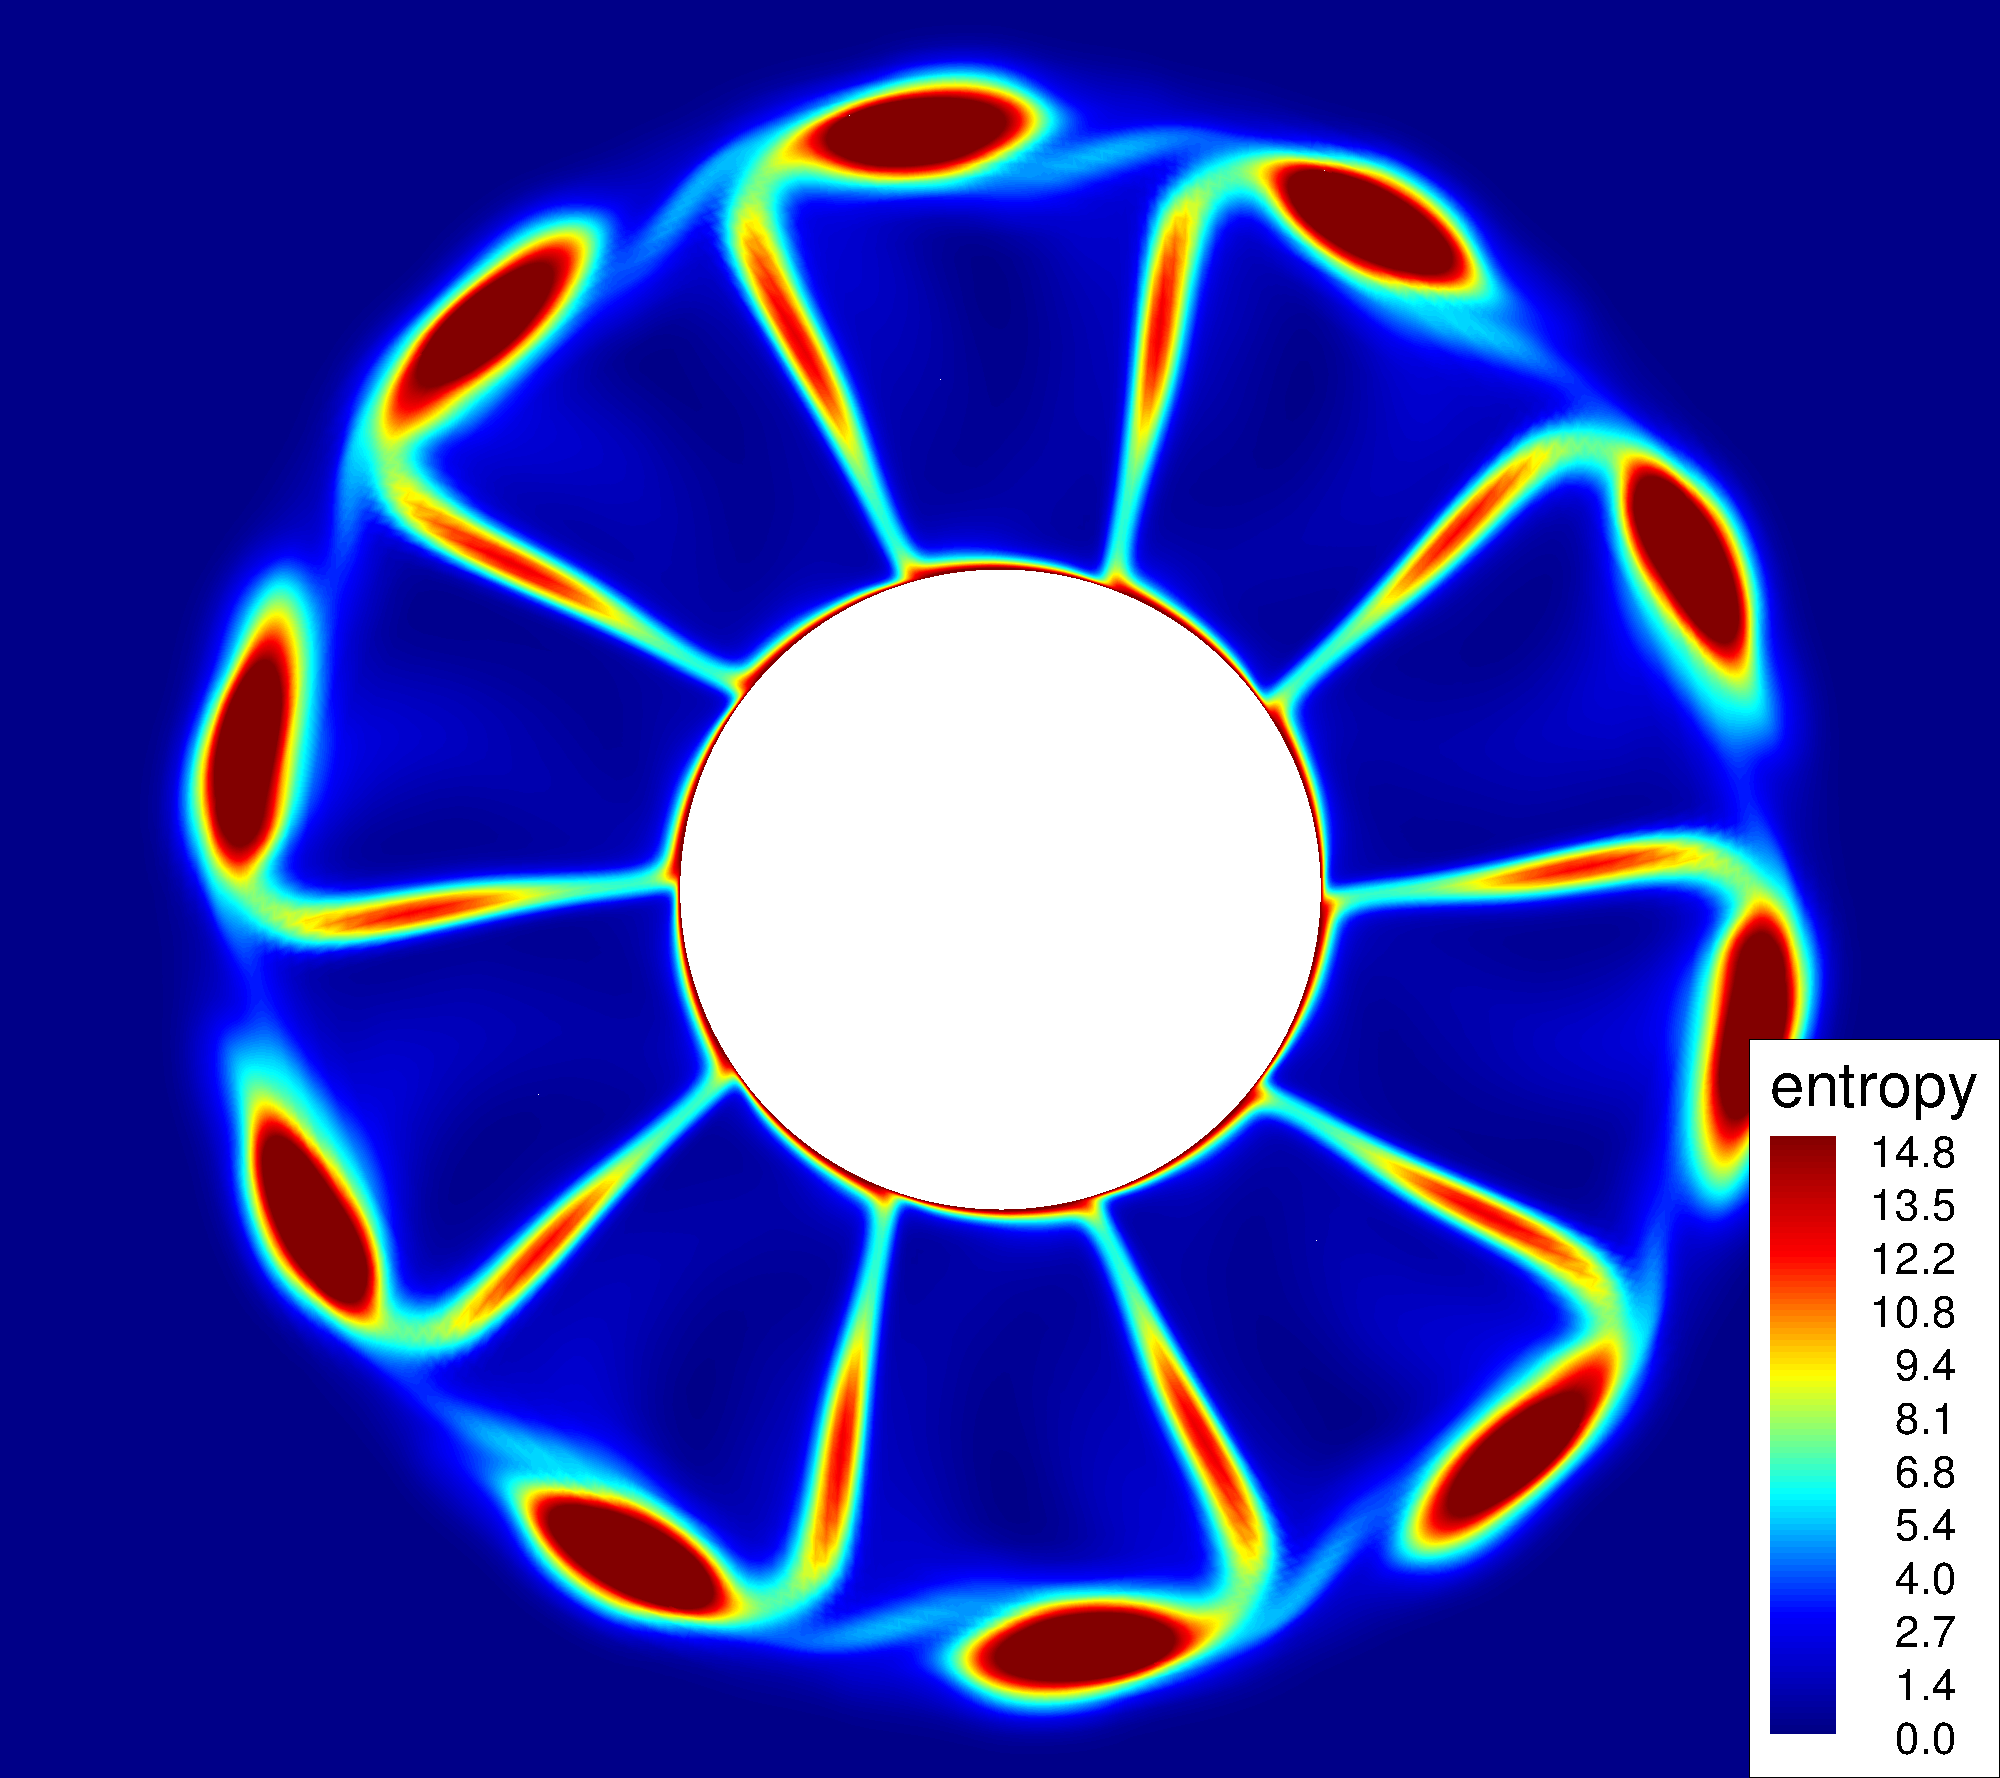
\includegraphics[width=.35\textwidth]{DREAM_LS_TSM_N4_roe2_sa_slice_x_rear_2_entropy.png}}
  \caption{Low-speed isolated configuration: axial cuts of entropy.}
   \label{fig:dream_ls_hb_axial_cut_entropy}
\end{figure}

\subsection{Two-dimensional results: radial cut of harmonic pressure}
\label{sub:dream_ls_hb_radial_cuts}

To further analyze the unsteadinesses that are seen
in a CROR configuration, a radial cut at 75\% of the
rear rotor height of the first harmonic
of the static pressure is show in 
Fig.~\ref{fig:dream_ls_hb_radial_cuts}.
The two rotors rotating in opposite direction, a steady
field for the former is seen as unsteady by the latter and \emph{vice-versa}.
Therefore the flow field is, by nature, discontinuous at the rows interface.
\begin{figure}[htp]
  \centering
  \includegraphics*[width=0.40\textwidth]{DREAM_LS_TSM_N4_roe2_sa_slice_r_70_ps.png}
  \caption{Low-speed isolated configuration: radial cut of the first harmonic of the
  static pressure normalized by the inflow static pressure.}
  \label{fig:dream_ls_hb_radial_cuts}
\end{figure}

On the front rotor side of the interface, a high amplitude azimuthal 
pattern of static pressure is seen. It is representative
of the potential effects: the blades deviates the stream lines and
as the two rotors rotate in opposite directions, theses deviations
are finally seen as unsteady flow features, hence the observed high amplitude.

On the rear rotor side of the interface, no azimuthal pattern 
of static pressure is observed near the interface.
Conversely, the pressure unsteadinesses are mostly observed near the rear rotor blades.
These pressure unsteadinesses come actually from the unsteady wake passing.
In fact, the absolute velocity deficit in the wakes shed by the front rotor
is seen as unsteady by the rear rotor. However, at the blade walls,
the velocity is necessary null. These 
velocity fluctuations are actually seen as pressure fluctuations since the presence
of the blades transforms velocity into pressure at blade walls.
Figure~\ref{fig:dream_ls_hb_radial_cuts_machrel}
supports this argument as the amplitude of the Mach number fluctuations
vanishes in regions where the pressure fluctuations grows.
\begin{figure}[htp]
  \centering
  \includegraphics*[width=0.40\textwidth]{DREAM_LS_TSM_N4_roe2_sa_slice_r_70_machrel.png}
  \caption{Low-speed isolated configuration: radial cut of the first harmonic of the
  relative Mach number.}
  \label{fig:dream_ls_hb_radial_cuts_machrel}
\end{figure}

